\section{Desenvolvimento}

Este capítulo detalha os processos que ocoreram no desenvolvimento da pesquisa, mostrando os passos seguidos para alcançar os objetivos propostos. Além disso, são abordadas as dificuldades enfrentadas e as adptações e refinamentos realizados ao longo do percurso.

\subsection{Circuito}

\subsubsection{Emissor}

O circuito que permite ``transformar" os bits em luz é composto por um led de alto brilho, um transistor TIP122, dois resistores e uma bateria.

O transistor é ligado como chave na SBC para permitir acionar cargas elétricas da qual a SBC não seria capaz, pois pode fornecer no máximo 16 mA (miliampère) \citeonline{correnteSbc} e como o \textit{led} de alto brilho consome uma corrente de 18.8mA, uma ligação direta na GPIO (\textit{General Purpose Input/Output}) poderia queimar a SBC.

\begin{figure}[!htbp]
  \caption{Esquema do circuito emissor}
  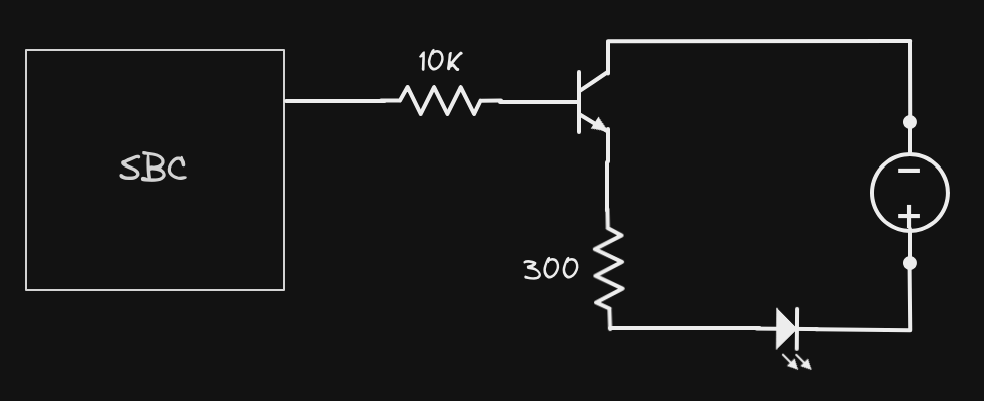
\includegraphics[width=0.5\textwidth]{images/esquema_circuito_emisor.png}
  \legend{Fonte: Autor (2023)}
  \label{esquema-circuito-emissor}
\end{figure}

\begin{figure}[!htbp]
  \caption{Foto do circuito emissor}
  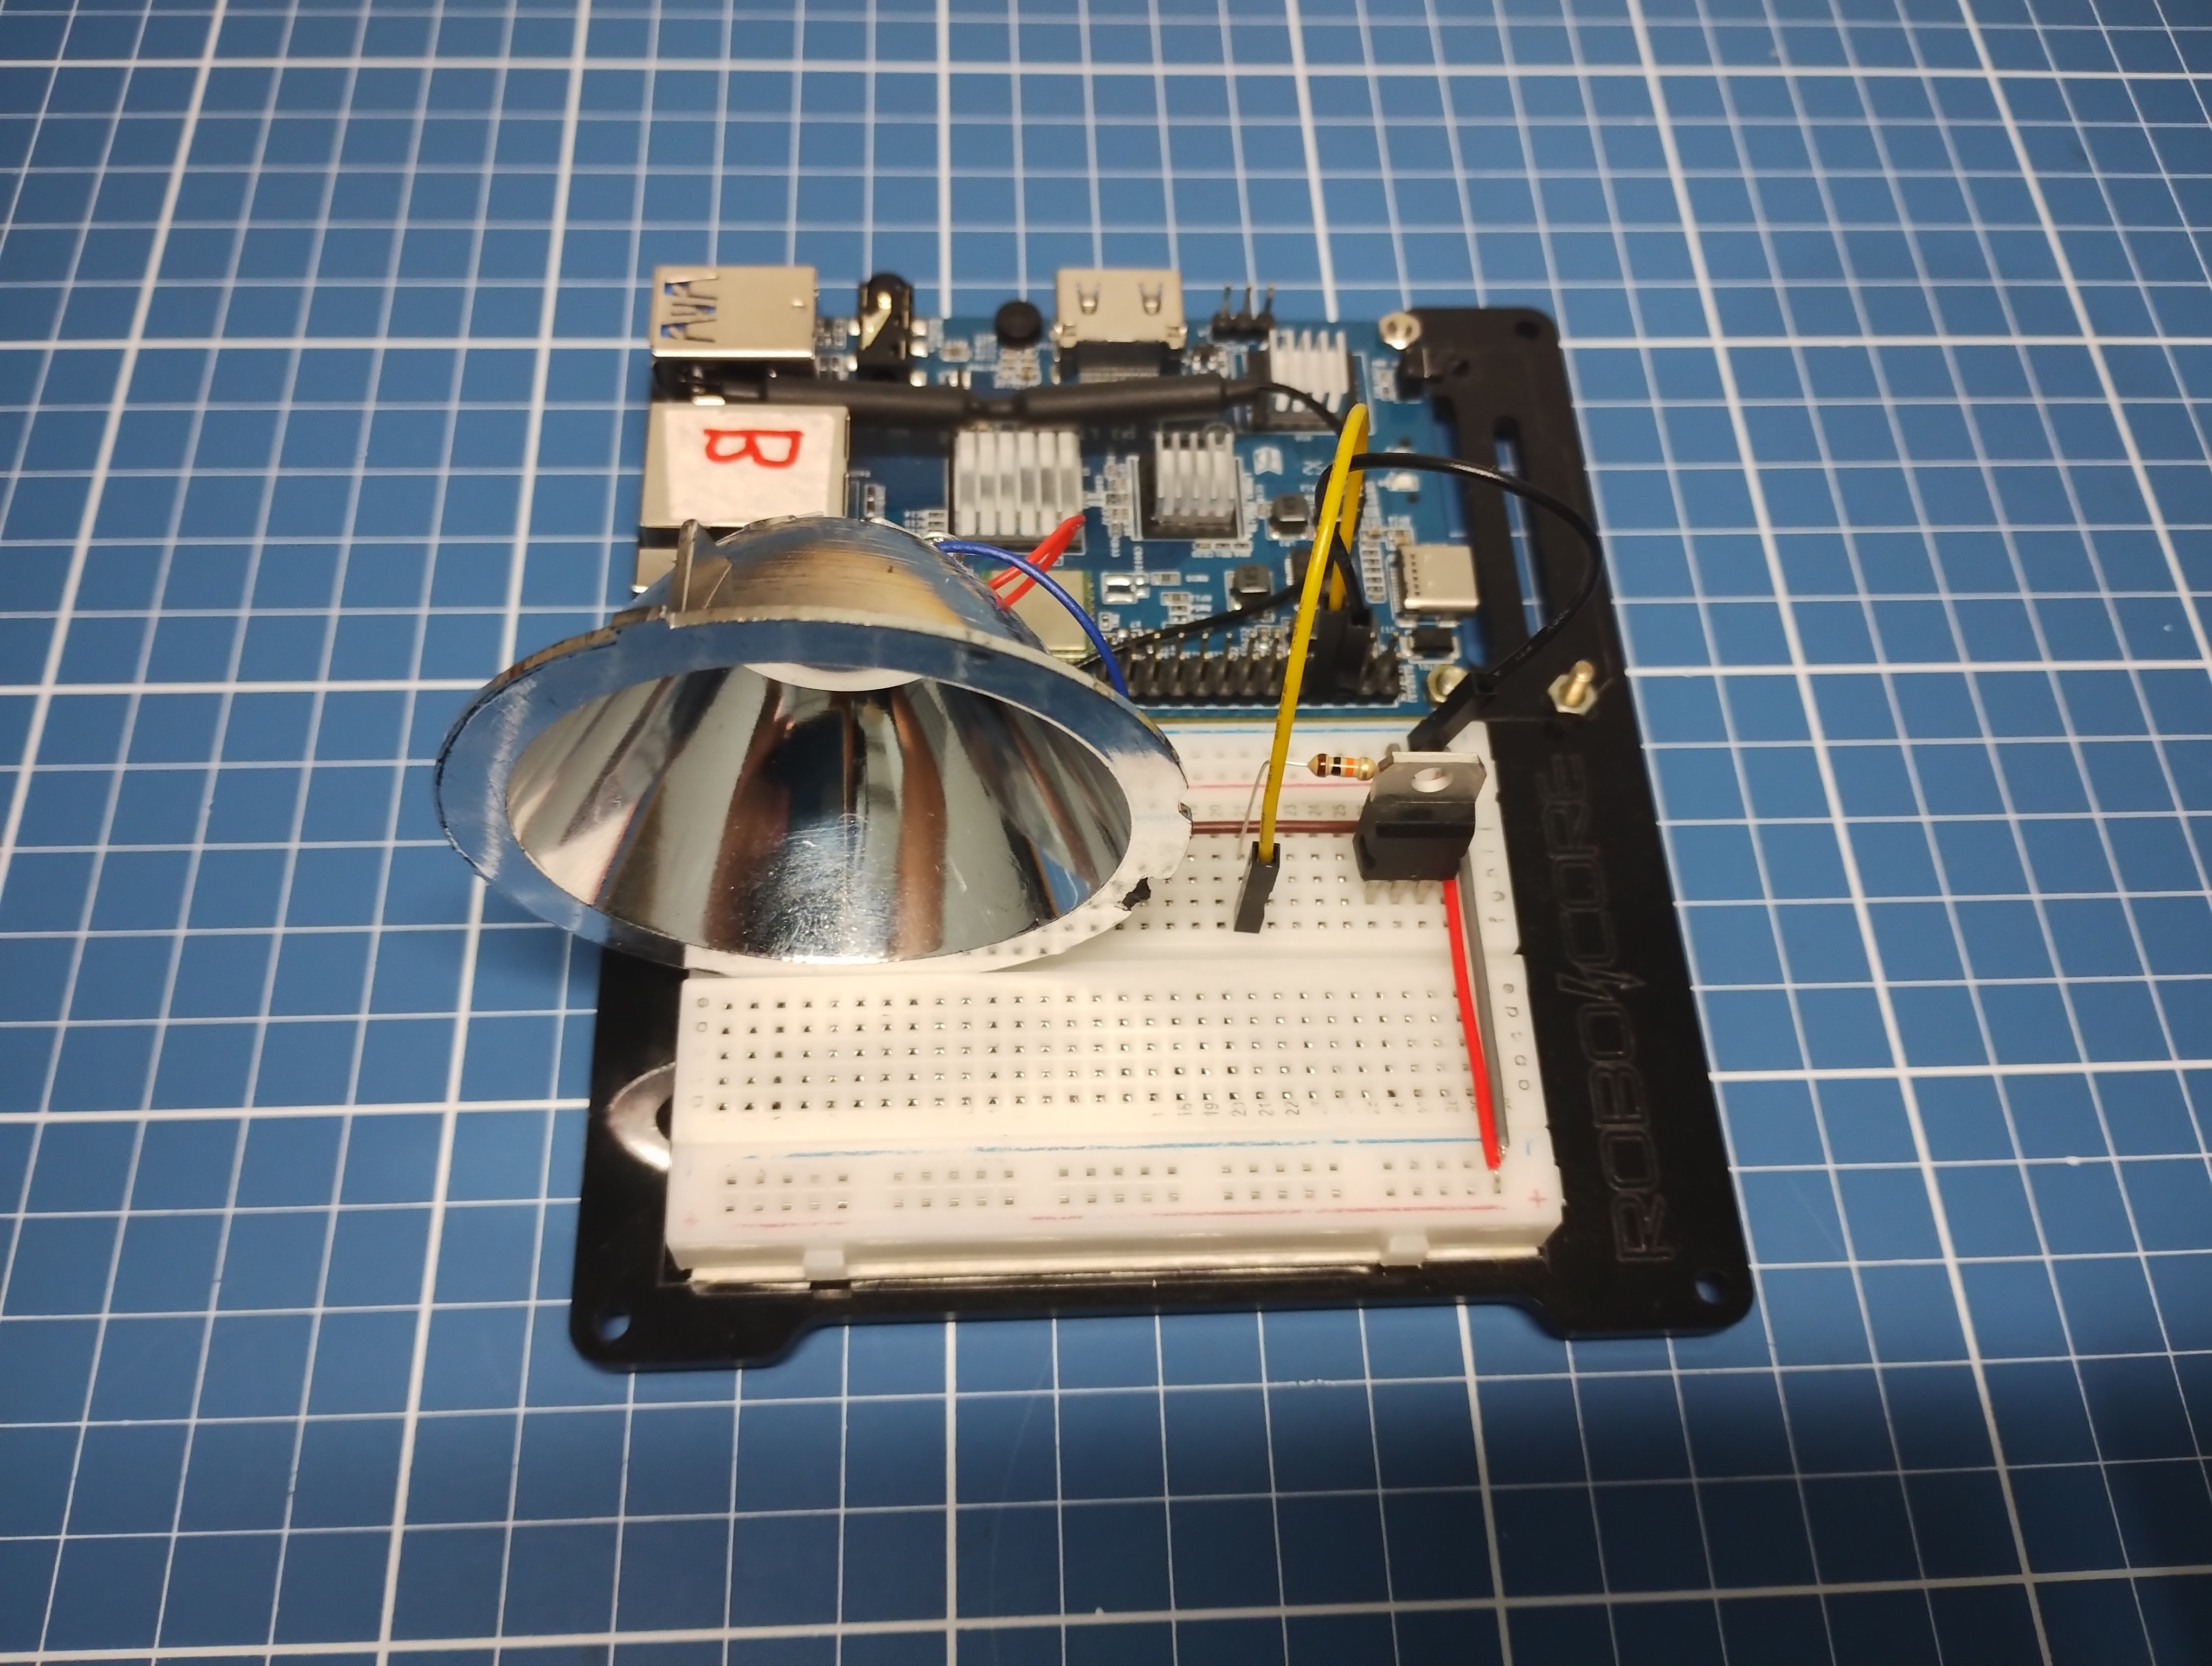
\includegraphics[width=0.4\textwidth]{images/foto_circuito_emisor.jpg}
  \legend{Fonte: Autor (2023)}
  \label{foto-circuito-emissor}
\end{figure}

\begin{figure}[!htbp]
  \caption{Consumo do \textit{led} usado no circuito emissor}
  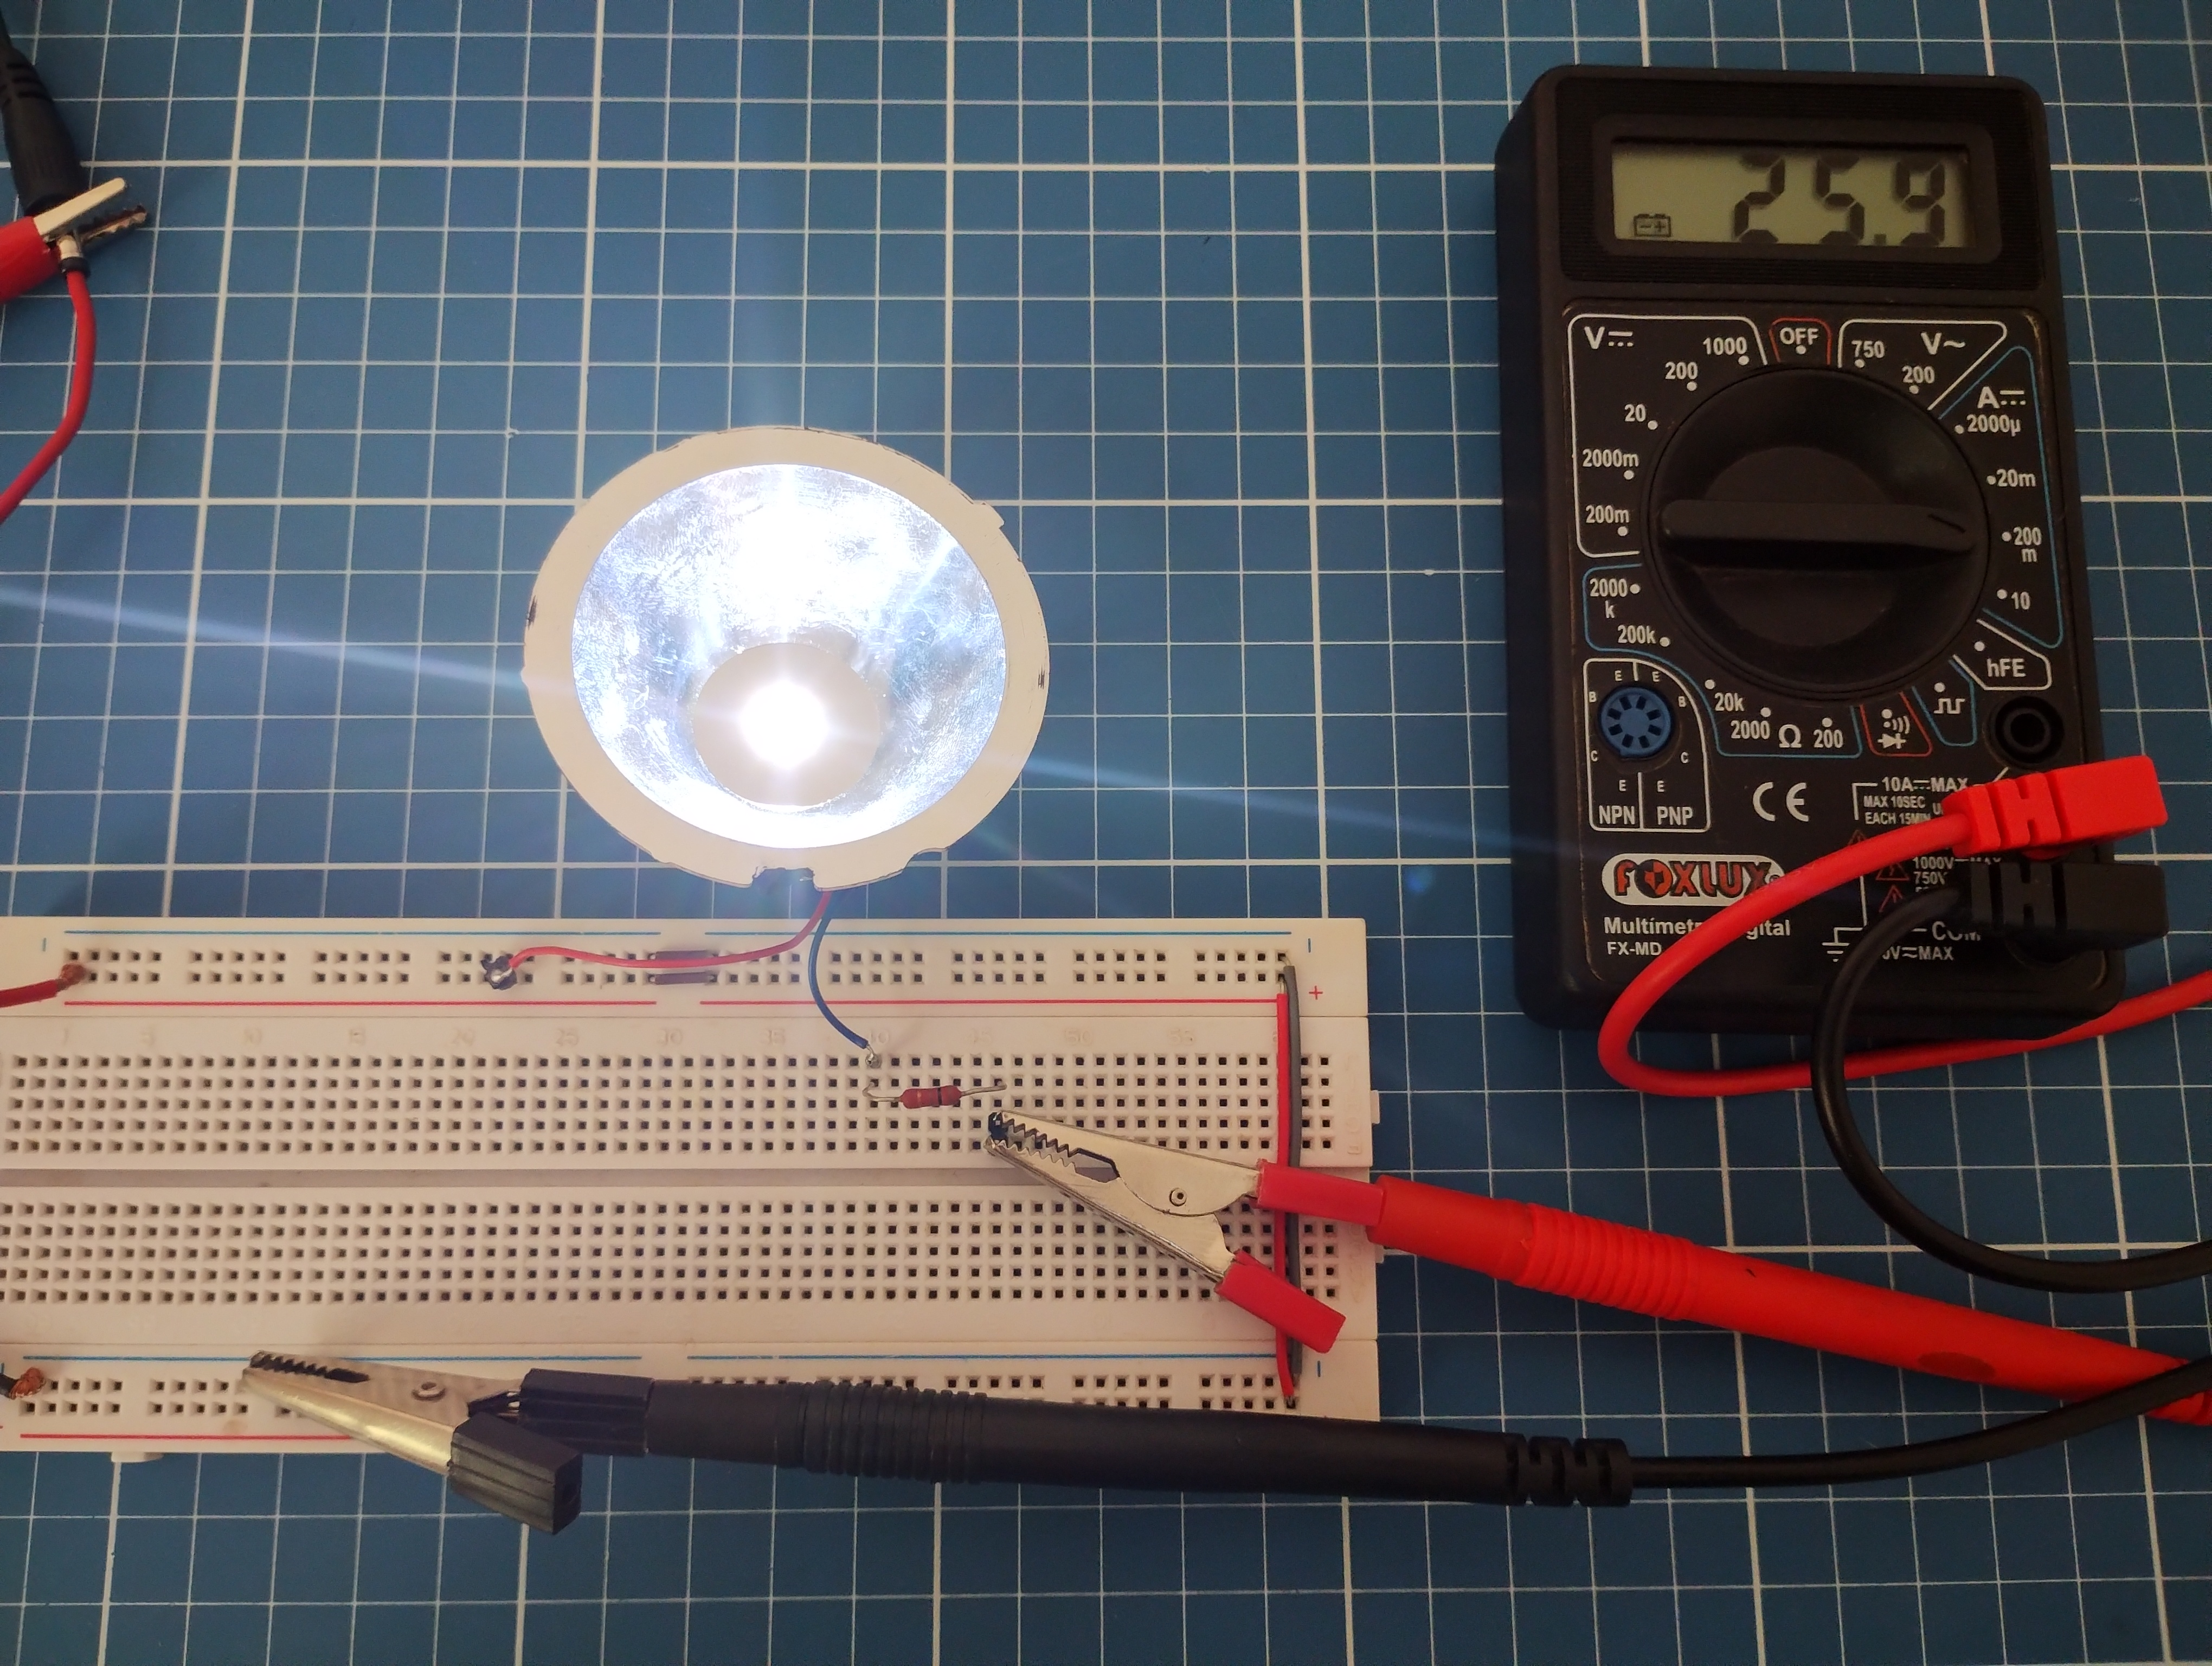
\includegraphics[width=0.4\textwidth]{images/consumo_led.jpg}
  \legend{Fonte: Autor (2023)}
  \label{corrente_led}
\end{figure}


\subsubsection{Receptor}

O circuito para receber as informações do emissor é composto por um LDR (\textit{Light Dependent Resistor}) e um potenciômetro ligado em série. Este circuito permite estabelecer uma faixa de corte de acordo com o nível de luminosidade do ambiente.

Estabelecido a faixa de corte ajustando o potenciômetro é possível "perceber" quando se está em nível lógico alto (bit 1) ou em nível lógico baixo (bit 0).


\begin{figure}[!htbp]
  \caption{Esquema do circuito receptor}
  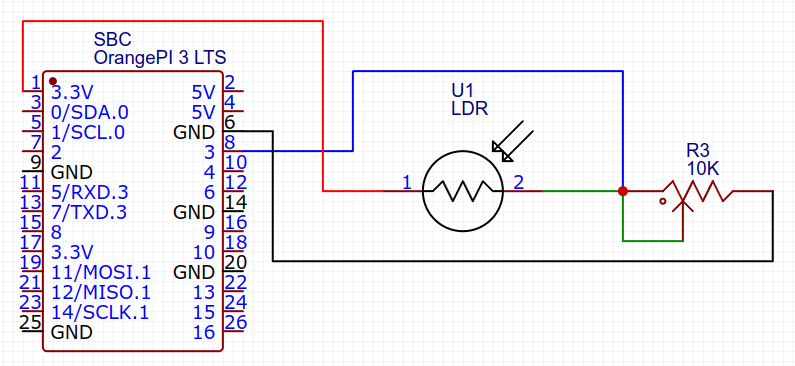
\includegraphics[width=0.5\textwidth]{images/esquema_circuito_receptor.png}
  \legend{Fonte: Autor (2023)}
  \label{esquema-circuito-receptor}
\end{figure}


\begin{figure}[!htbp]
  \caption{Foto do circuito receptor}
  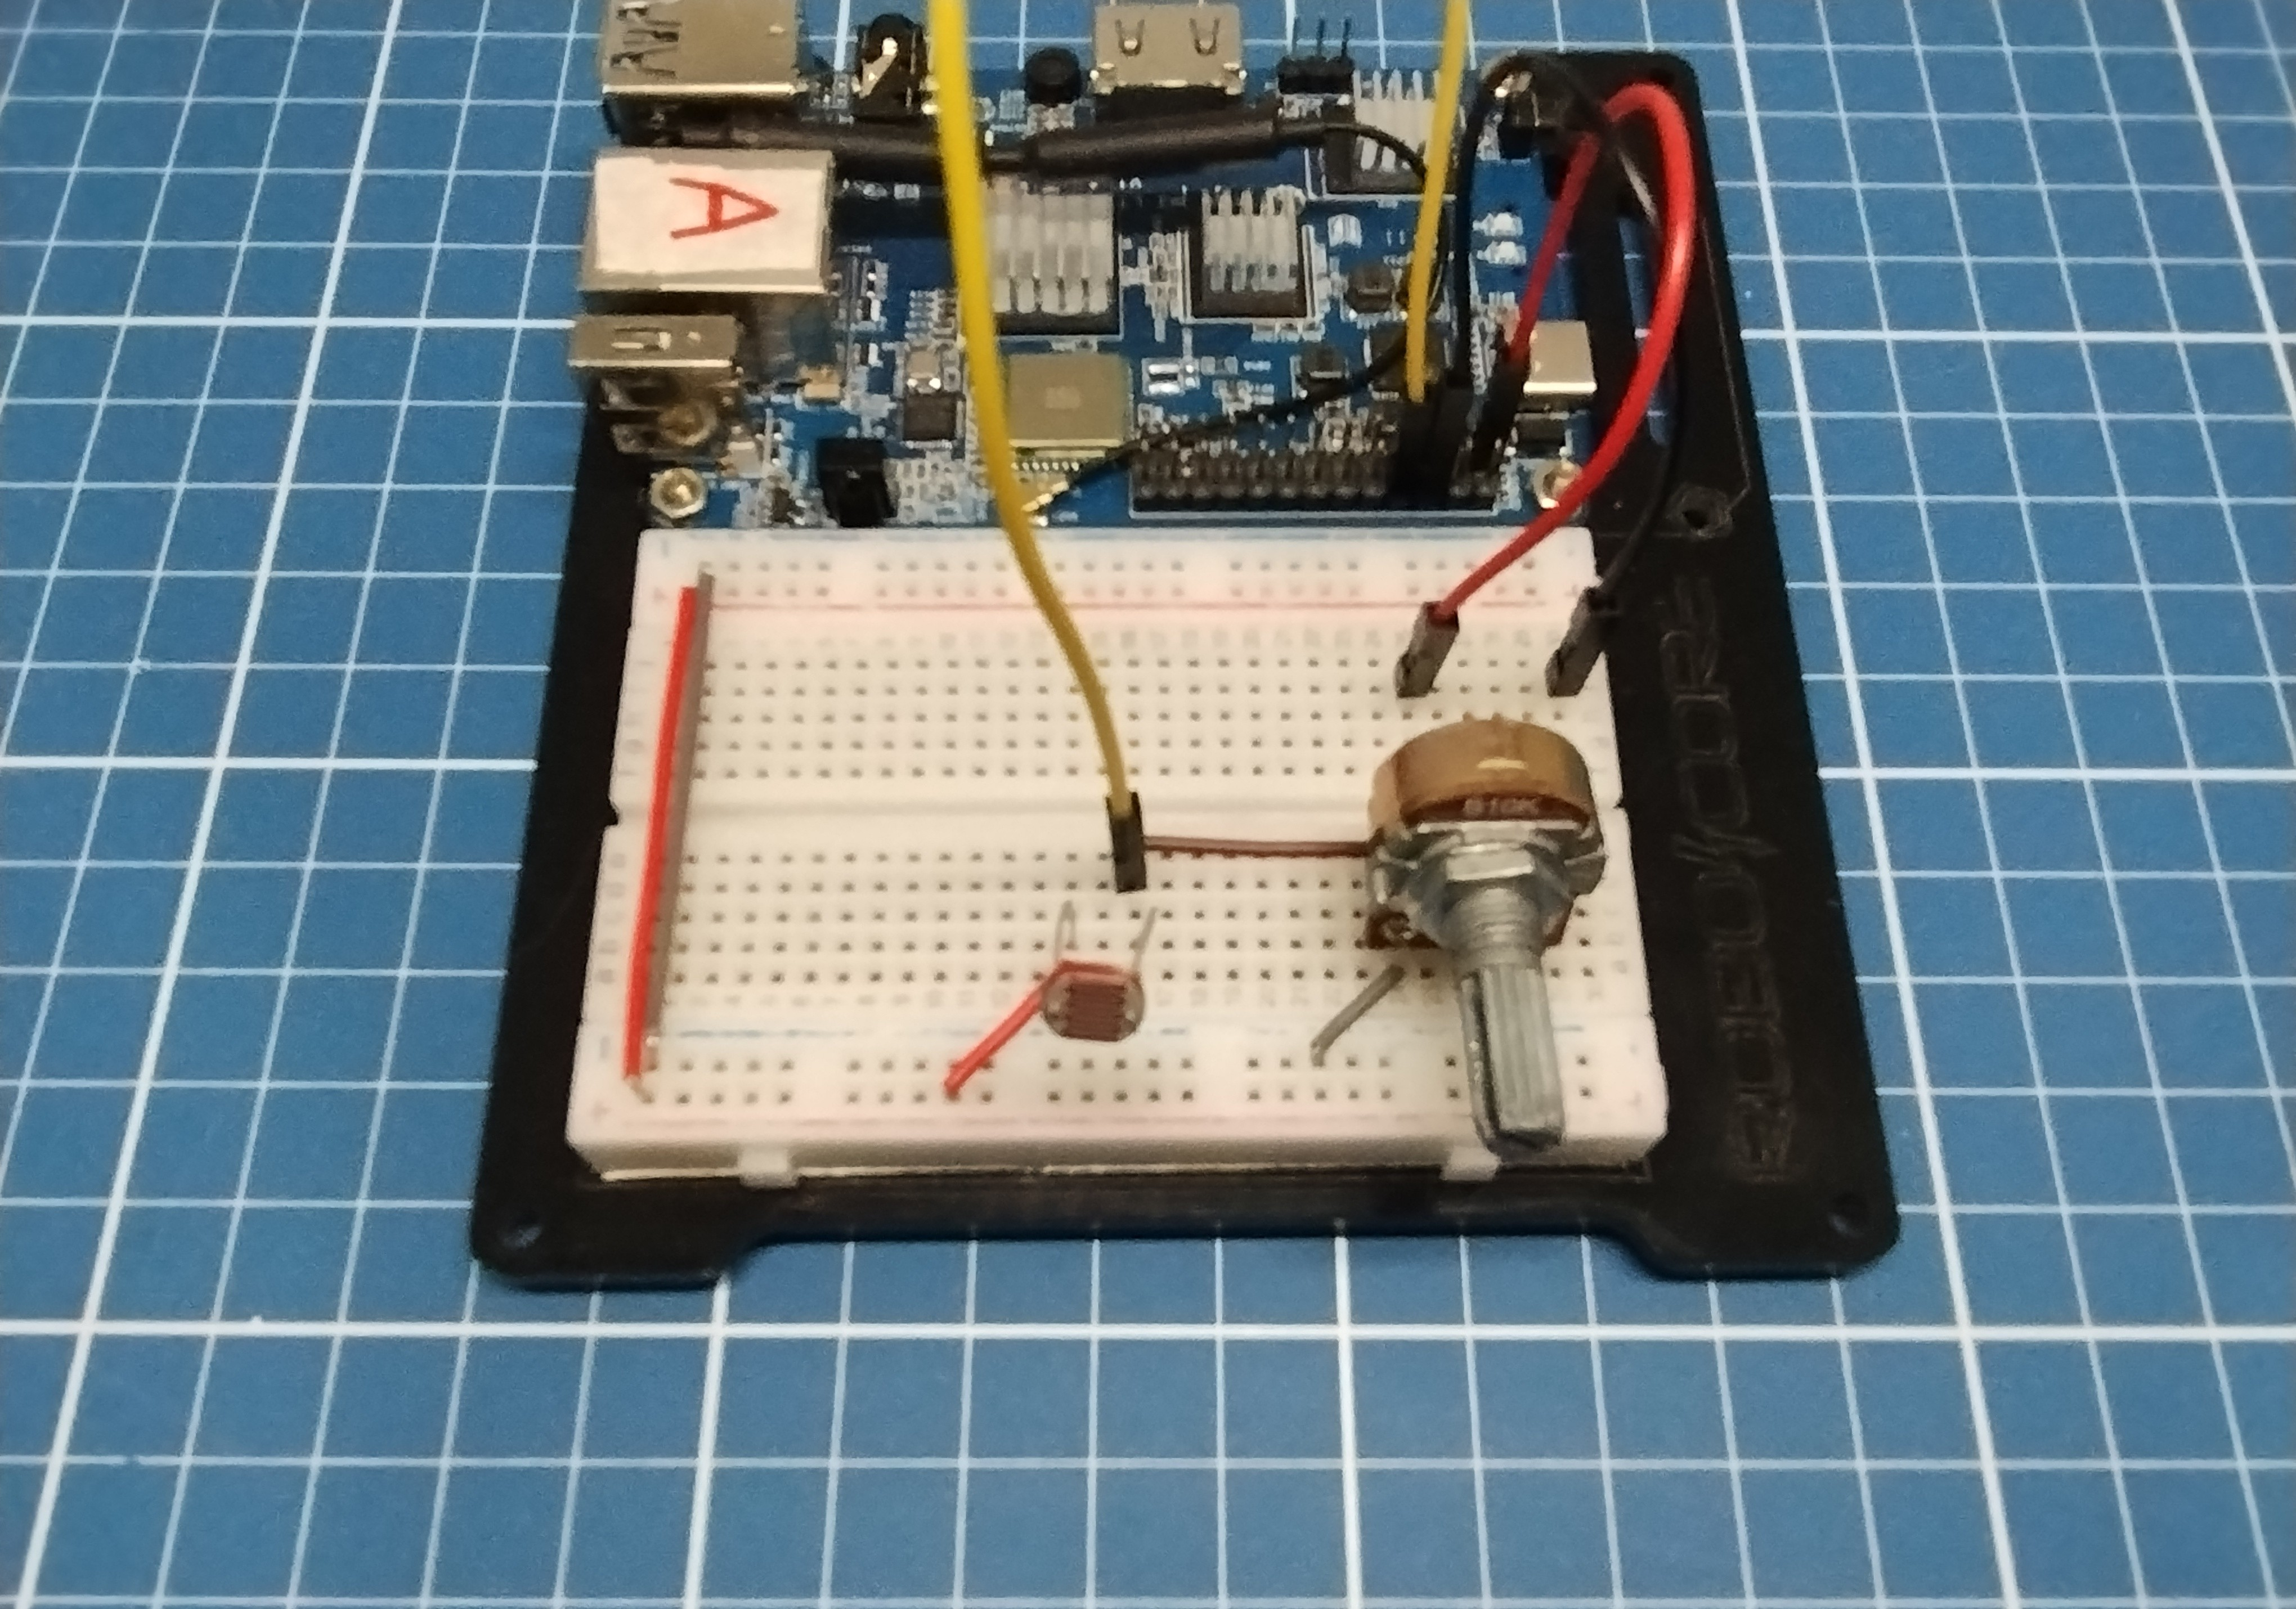
\includegraphics[width=0.4\textwidth]{images/foto_circuito_receptor.jpg}
  \legend{Fonte: Autor (2023)}
  \label{foto-circuito-receptor}
\end{figure}

\subsection{Software}

O código foi implementado nas SBCs usando a biblioteca \textit{wiringPi} e \textit{wiringOP}, que é um \textit{fork} da \textit{wiringPi} para a \textit{OrangePi}. O \textit{software} implementa um protocolo de comunicação chamado de \textit{start-stop}, que consiste em uma forma de sinalizar o iníco e o fim de uma transmissão de dados. No início, é eviado um bit de \textit{"start"} indicando o início da transmissão seguido dos dados e por fim um bit de \textit{"stop"} indicando o fim.

